\chapter{Testbeam}
\label{c:Testbeam}

The Baby MIND collaboration performed an electronics validation using a Totally Active Scintillating Detector (TASD) at the T9 test beam in the PS facility at CERN in 2016. After construction was completed In 2017, the full Baby MIND was commissioned in the same test beam.

The Baby MIND test beams tests took place at the T9 beam line at the proton synchrotron (PS) experimental hall. The beam lines are derived from the 24 GeV/c primary proton beam from the PS, which provides 2.4 s cycles of about 400 ms spill duration. The T9 beam comes of as a secondary beam by firing the proton beam at a 200 mm thick Aluminum target which delivers secondary particles up to 15 GeV/c at a production angle of 0 degrees. The line is designed to provide the users with non-separated secondary particles, with positive or negative polarity, as hadron (pion) or muons and the beam momentum can be adjusted by setting the currents for the optical magnets of the beam line.

In this section details will be given to how data is collected and processed before showing some sample events and then further describe how data is processed in SaRoMaN to provide results obtained from each of the two test beams.

%Write like a lab report, describe what we are doing with T9, what is happening in the detector when a particle comes through, what happens with the data and how it is saved. When this is saved, what does the unpacking do and SaRoMaN. After all of this, how is the analysis done, what are the plots etc etc.

\section{TASD-testbeam}

\subsection{Setup}
During June-July 2016 a test beam was performed to characterise the readout system, data acquisition (DAQ) and electronics to be used in the Baby MIND detector. The test beam was at the T9 beam of the East Area, operating at the Proton Synchrotron (PS) at CERN. A Totally Active Scintillation Detector (TASD) constructed under the AIDA-2020 project (Advanced European Infrastructures for Detectors at Accelerators) was used to test the readout system, electronics, DAQ and reconstruction software.

The TASD detector consisted of horizontal and vertical planes, each plane with 16 scintillator bars, $10\times10\times1000 mm^3$, and can be~\FigRef{fig:TASD}. Each bar is read read out on both sides by S12571-025C Hamamatsu Multi Pixel Photon Counters (MPPCs). There are a total of twelve planes of either horizontal or vertical type in an alternating vertical, horizontal pattern. The layout is six combined planes providing both vertical and horizontal information with spacing between each. This summarizes as a detector with 96 horizontal and 96 vertical bars read out on both sides using a total of 384 MPPCs and a total size of $1m^3$. Check and mention uninstrumented bars? Gap size? Etc. Etc. A real life figure?

\begin{figure}[h!]
\centering
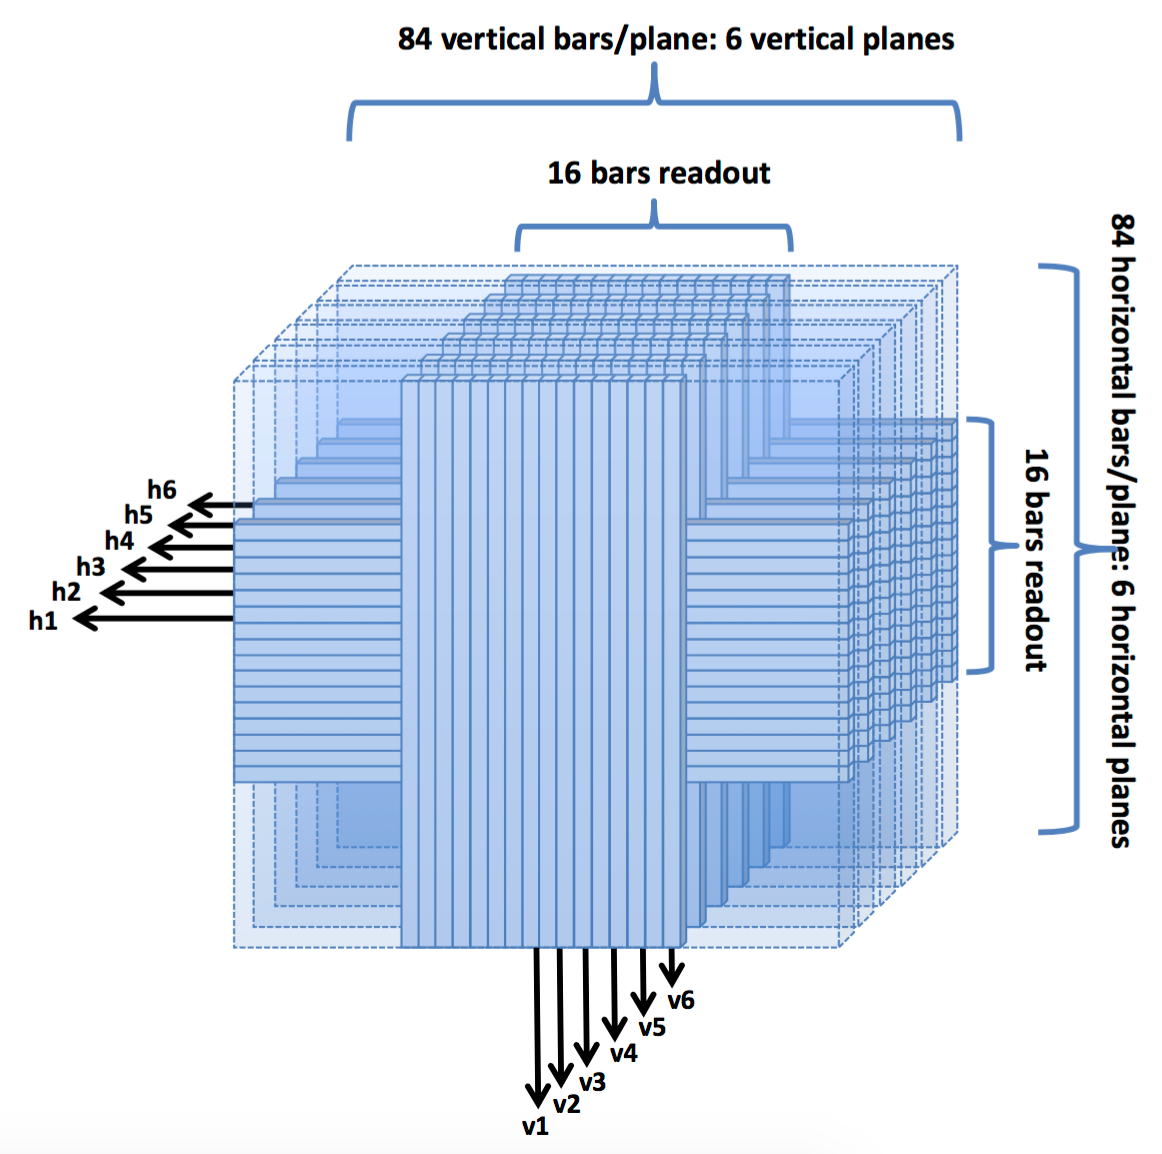
\includegraphics[width=0.5\textwidth]{figures/AIDA.png}
\caption{The TASD with the instrumented bars visualised}
\label{fig:TASD}
\end{figure}

\subsection{DAQ}
Each MPPC is connected to a Front End Board (FEB) which returns data in a specific format. For the setup a full 4 FEBs were used each able to read 96 MPPC channels each. These FEBs were then all connected via USB3 to a readout PC. 

During the initial test beam FEBv1 was used. For, ease in finding plots, details regarding FEBv2 are going to be shown.
\textbf{Readout format and block chart can be seen in figures? }OR \cite{71Status17}.

This data is sent from each of the FEBs in a custom made data format. The data format simplifies combining the data from all of the FEBs, however it also 
only works for offline processing as the footers need to be read before any processing can be done.

When this is done an unpacking software is used to translate the format to actual usable data and hits. 

During the first test beam conversion between channel and position was hard coded, this was later changed to a database.  

\textbf{Describe how the data is read in, from the electronics etc etc. Mention that there is no real difference between TASD MIND beam daq. Only more! }

Described in some part in Baby MIND section hint at the readout block figure and describe how data is taken.  All in beam area. Signal created from particle depositing energy in bar, bar producing photons, photons measured by MPPC. MPPC produces an electrical signal which is sent to FEB, which samples the signals each 2.5 ns in gtriggers of 0.1ms, in spills given by the accelerator signal.

The FEB signals are sent to a back plane which sends the data several readout PC:s via USB.

Essentially that is how all the data is read out. The readout PC:s are controlled via remote connection/ethernet by a computer outside of the beam area in the control room.

The data is currently just recorded, thus all analysis needs to be handled offline. This is slightly due to the data format design, but also due to the complexity of the unpacking.

What is unpacking?

More details, limits, cuts, etc etc. What plots? Photo electron counts, dark counts, peaks. Very unusually good values. Bar efficiencies etc etc.

Describe how data is handled/used and combined after unpacking.

\subsection{Data preprocessing}
Describe how hits are handled and converted into the simulation format to be fully usable in the SaRoMaN framework.

Convert time and hits to x or y bar hits. These are then combined in the same way as for simulations. To remove excess events there are initial filters. Count hit places, potential for tracks? Remove potential pions? 

Mention that this is later lessened in the further analysis. (what I have done now).

Did not ans still do not have energy dep value.

\subsection{Results}

The main goal of this first test beam was to test the readout system, electronics, DAQ and reconstruction software. The results can be quite nicely summed up in \FigRef{fig:TASDres2} and \FigRef{fig:TASDres} and noting that the TASD was horizontally aligned but the beam was slightly off-center vertically. Detailed studies were performed and published in...


\begin{figure}[h!]
\centering
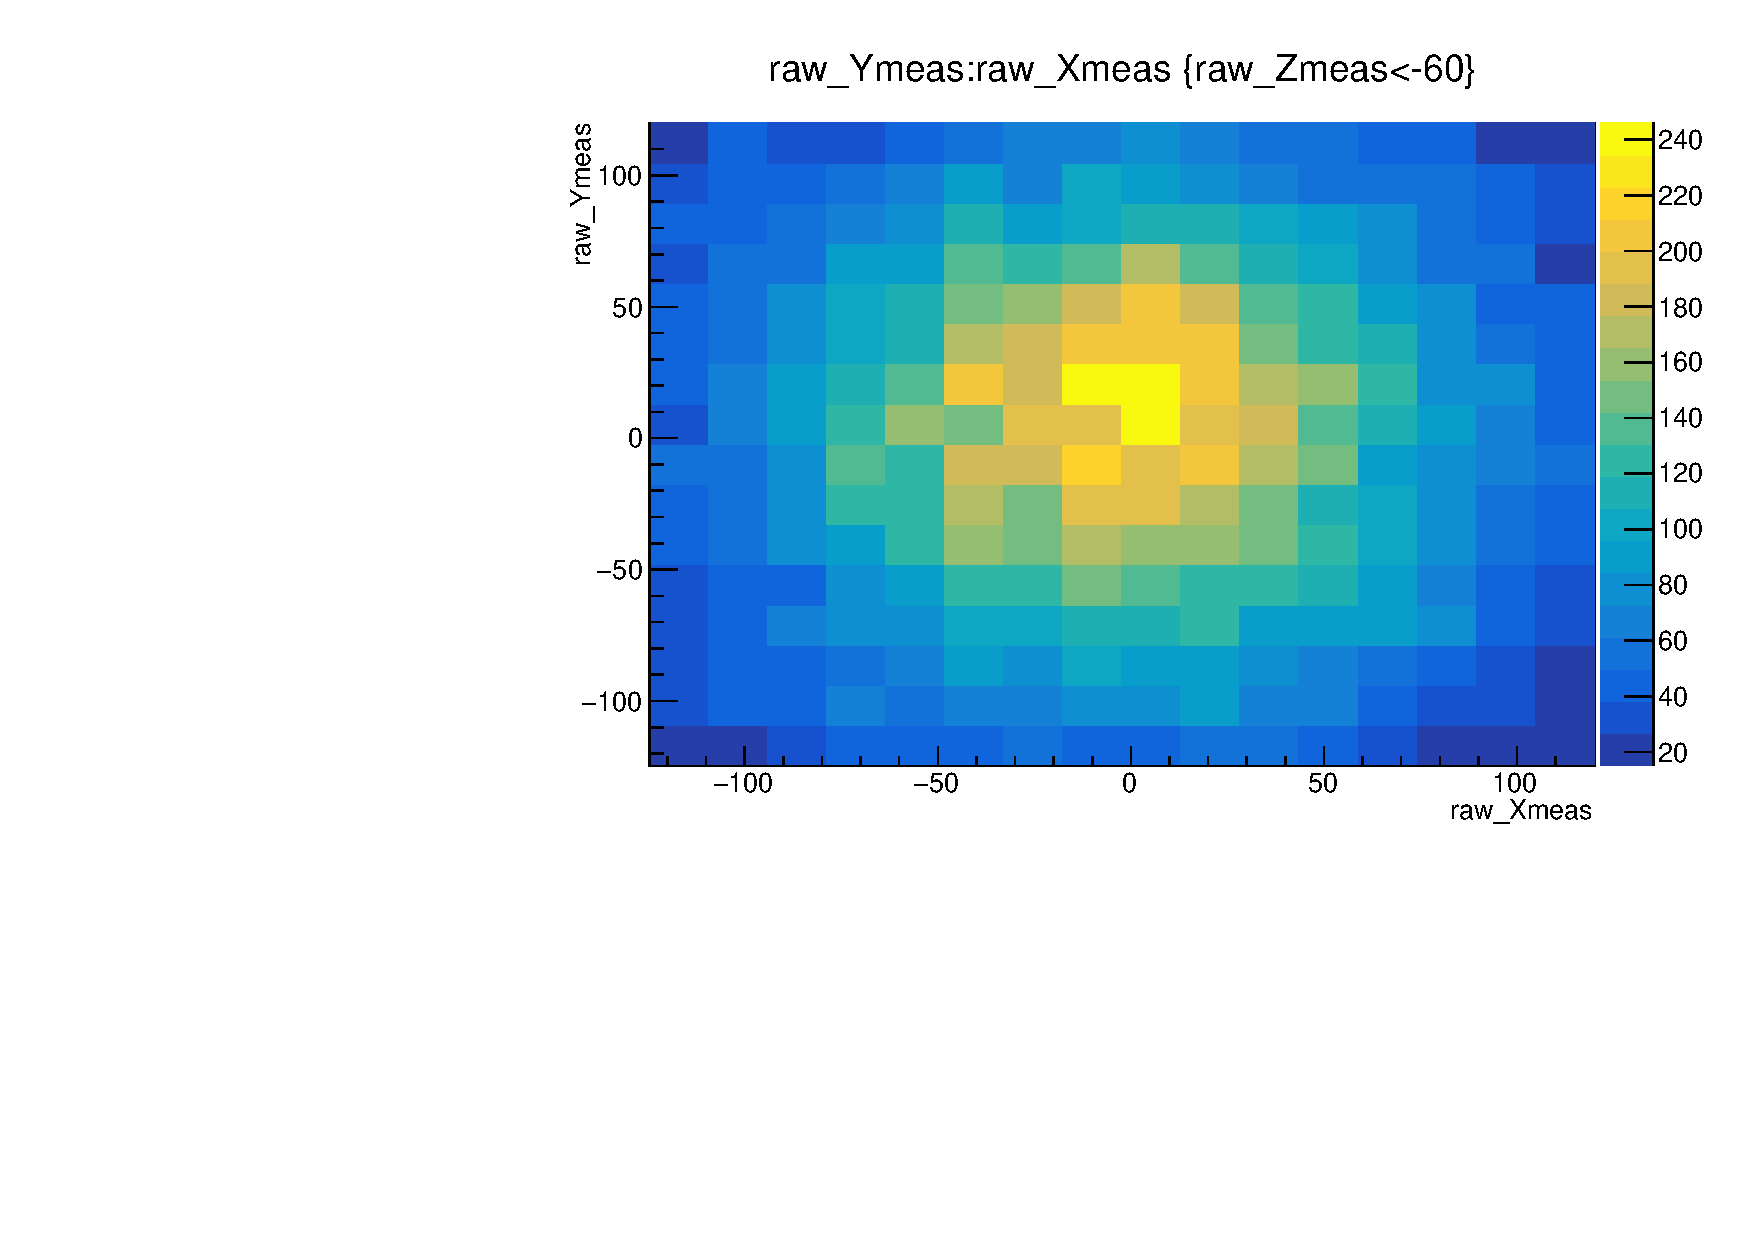
\includegraphics[width=0.48\textwidth]{figures/nuphys/newFigures/beamXYplane1Hadron.pdf}
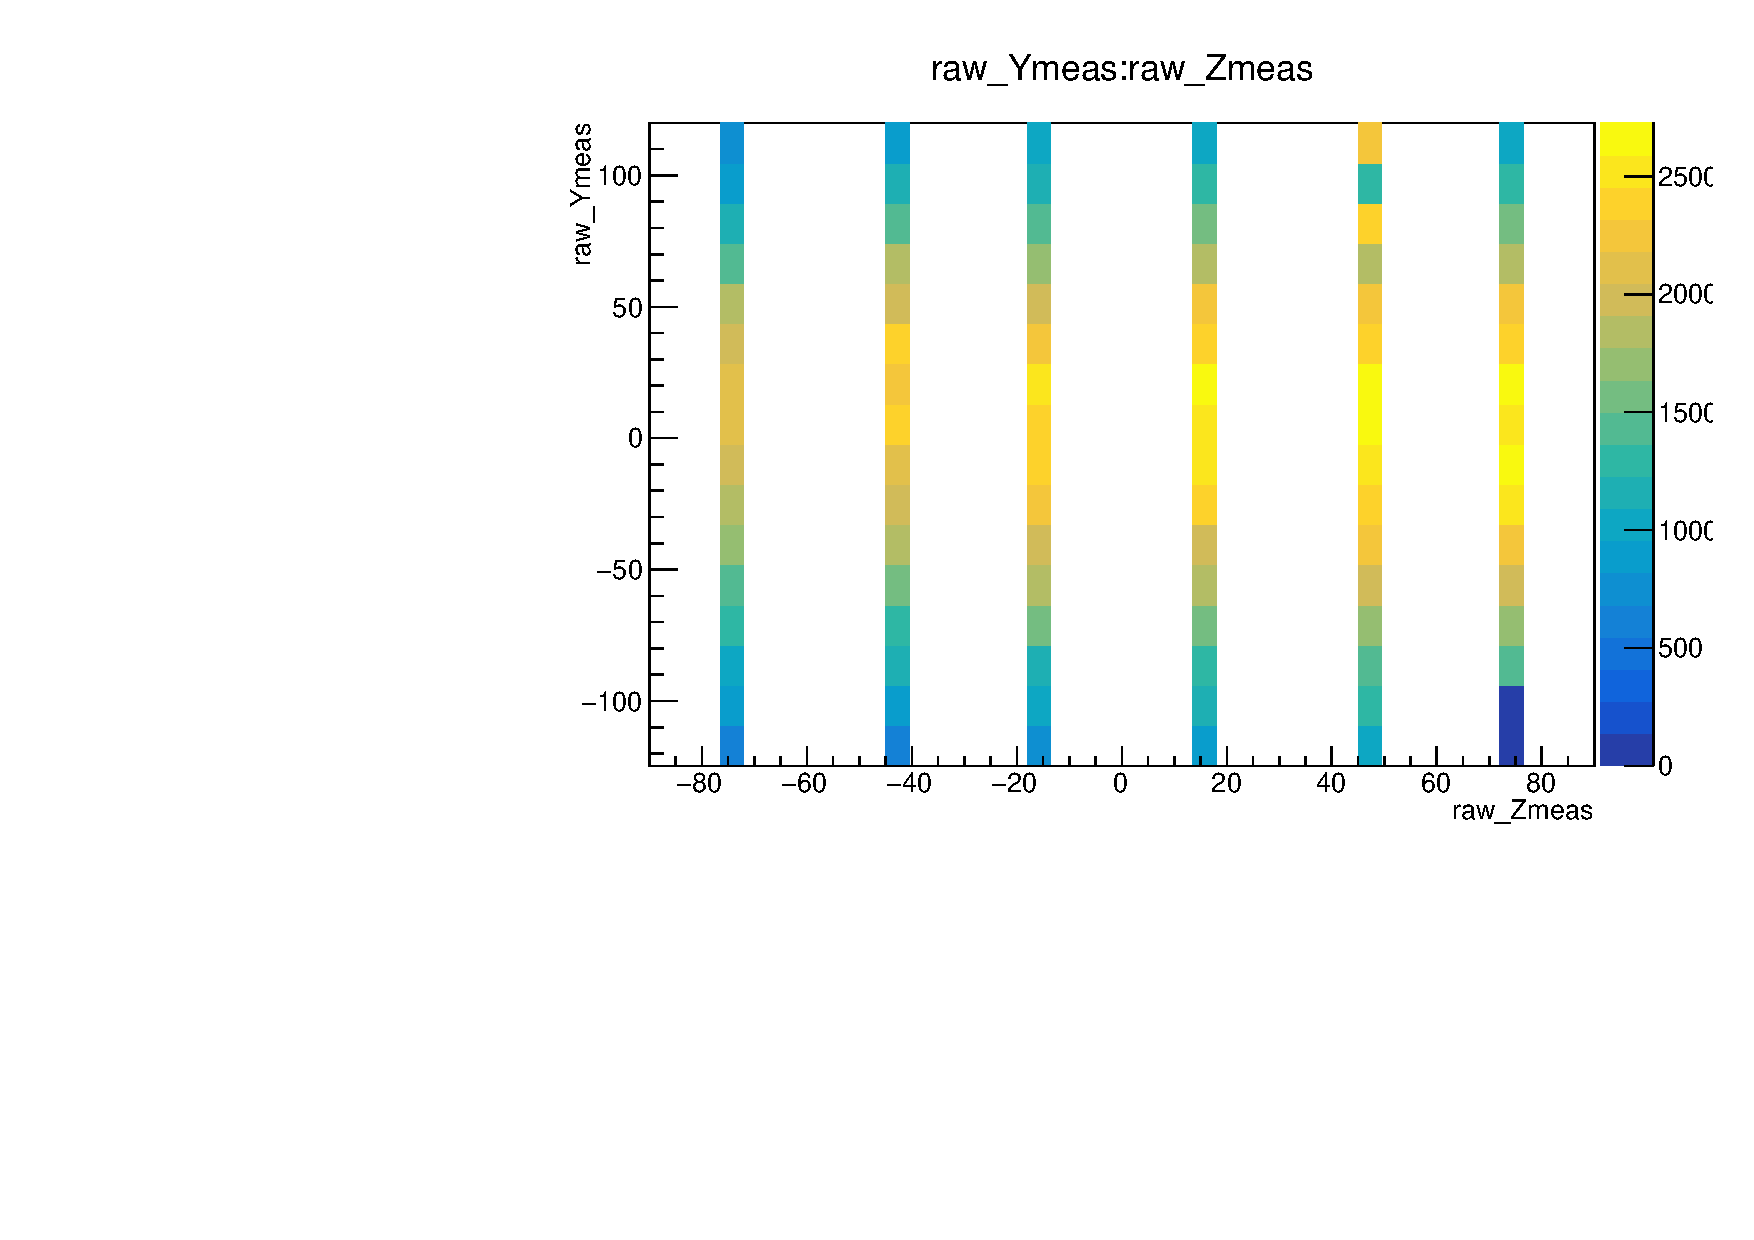
\includegraphics[width=0.48\textwidth]{figures/nuphys/newFigures/beamYZhadron.pdf}
\caption{(Left) An XY-beam profile as measured by the TASD. (Right) An YZ-beam profile as measured by the TASD}
\label{fig:TASDres2}
\end{figure}

\begin{figure}[h!]
\centering
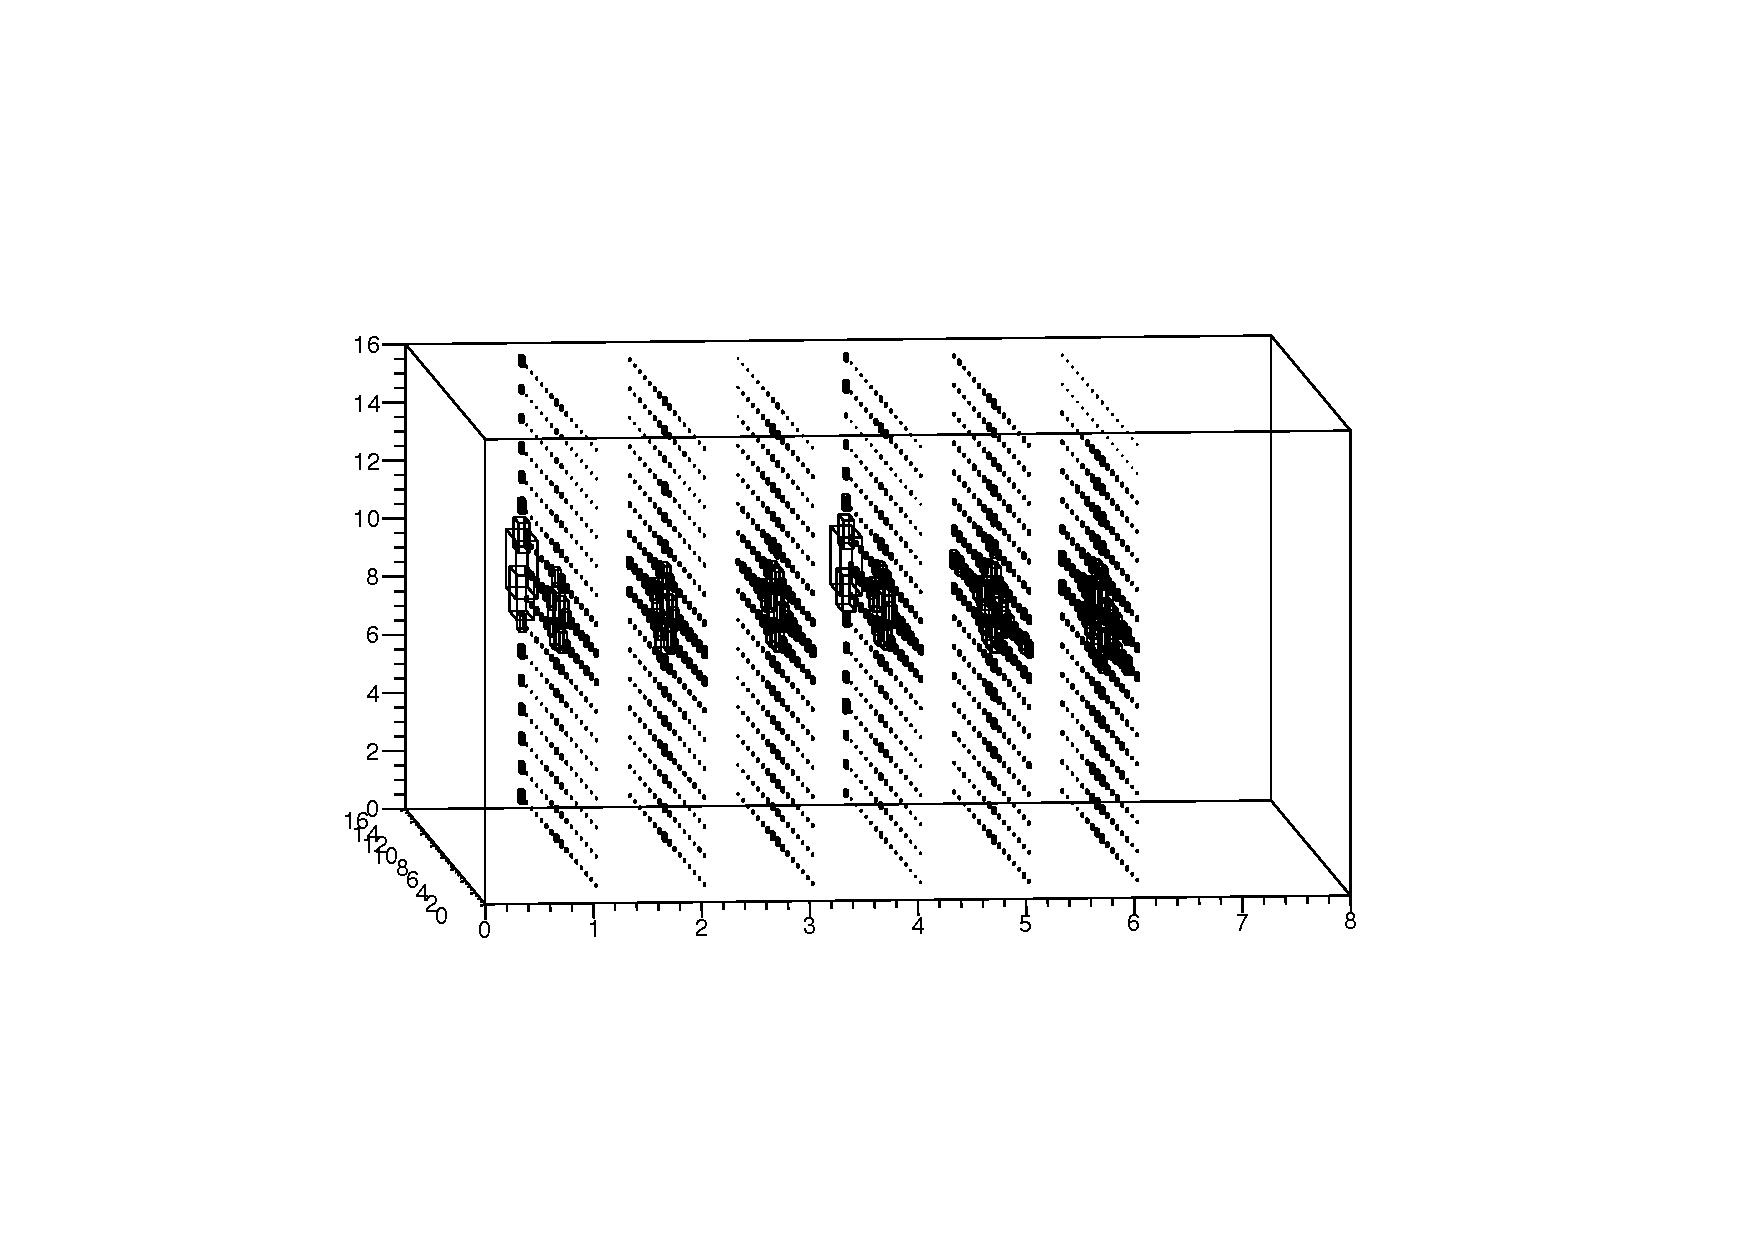
\includegraphics[width=0.48\textwidth,trim = 5cm 5cm 5cm 5cm]{figures/nuphys/newFigures/beamPlot.pdf}
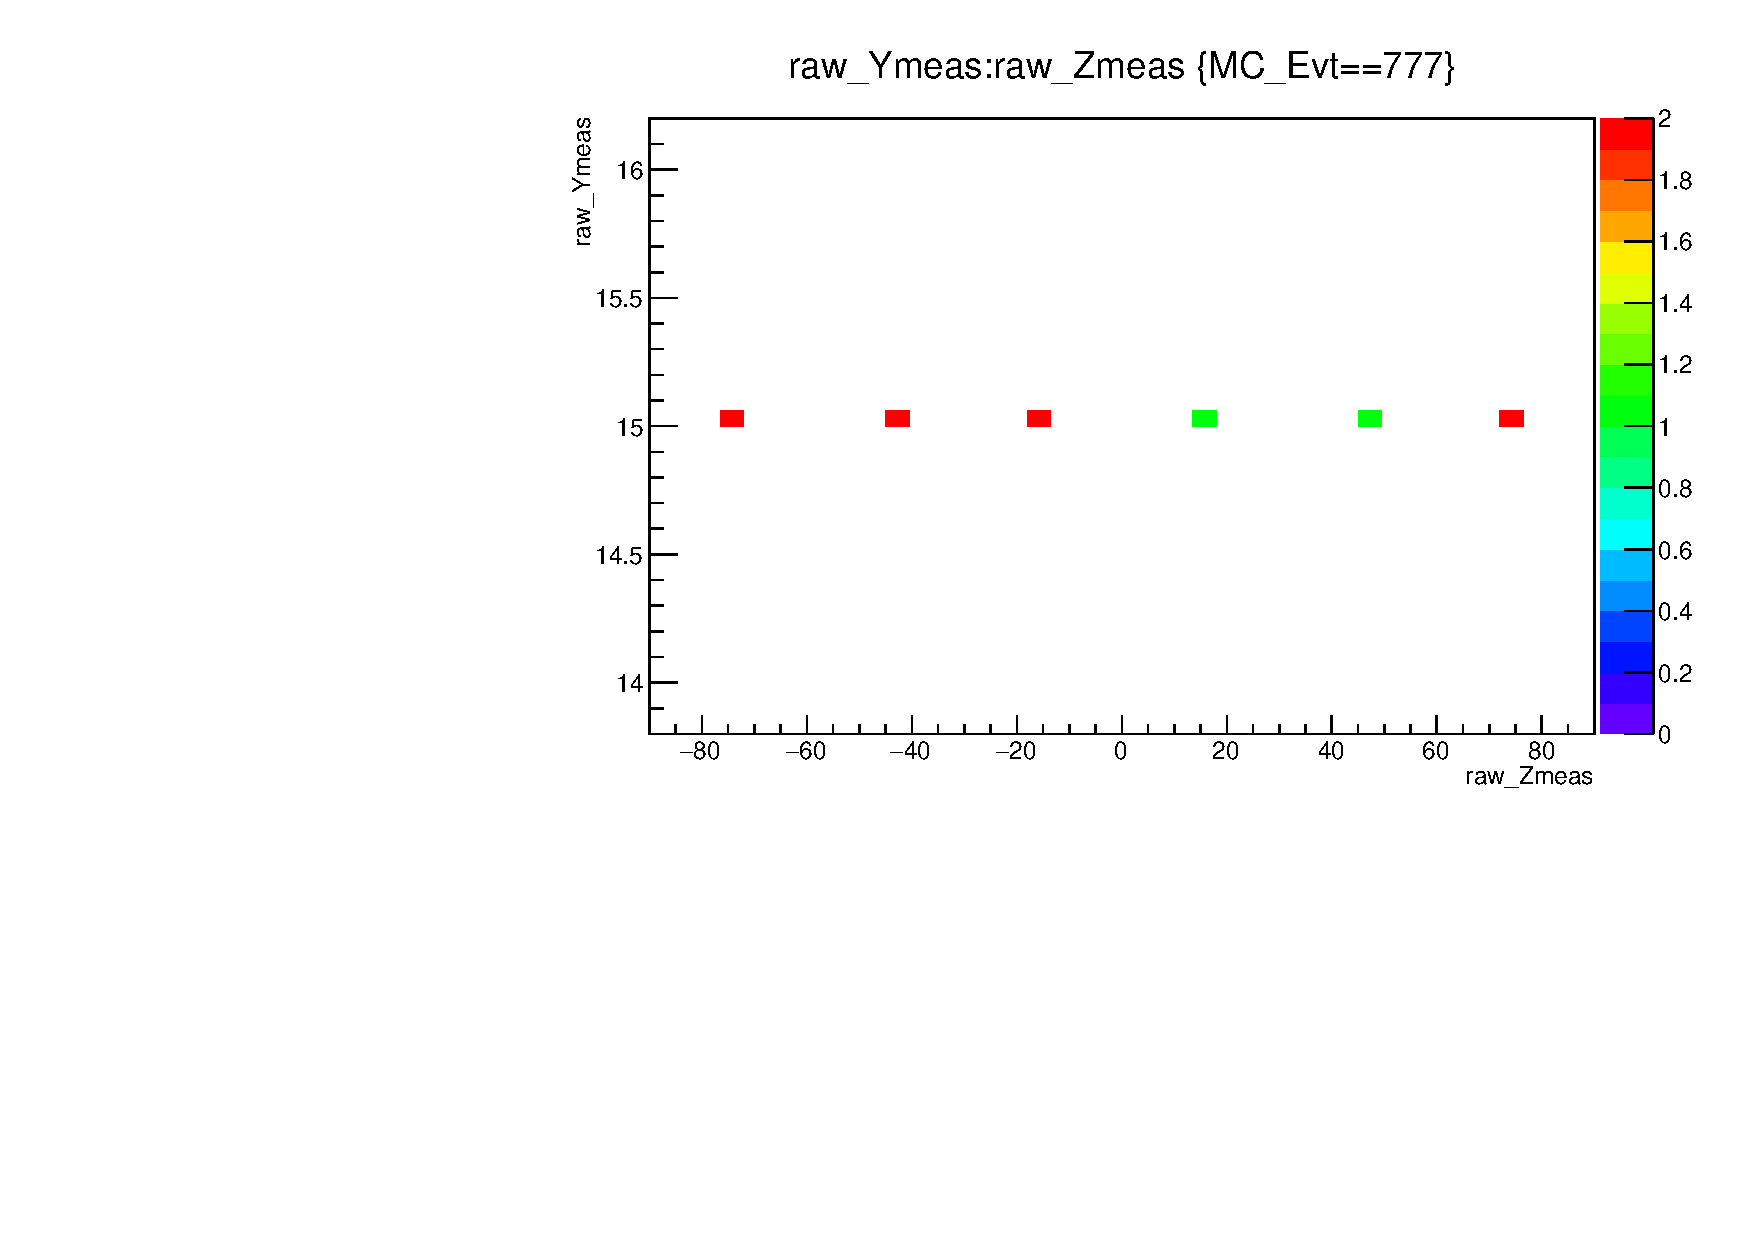
\includegraphics[width=0.48\textwidth]{figures/nuphys/newFigures/muonTrackYZ.pdf}
\caption{(Left) 3D-Beam profile measured by the TASD. (Right) Single muon track passing through the detector.}
\label{fig:TASDres1}
\end{figure}

Add in pion track?

What was lowest energy recorded in a bar? Results in lowest energy for horizontal and vertical.

The plots show both that the electronics and readout system works well, and that the data can be passed through the DAQ into the reconstruction software. Given that the TASD was only 6 planes of scintillator and did not have a magnetic field, the reconstruction software only combined hits in x and y with the z position to a final track, without being able to perform any momentum reconstruction. However it showed that the reconstruction software was operational and could create tracks from these hits.

Too few planes. No magnetic field. Confirms that the full chain works and can produce plots, however the results are slightly less than expected. Add in event displays. Something to show both pion showers and muons.

%What were the results, showed that the software seems to work, both digitisation and reconstruction. Anything else? All the electronics etc. Only result from me, plots on poster...  However this shows that software works well, compared slightly to simulations??? On hardware side, daq and full chain huge improvements. Went from nothing to ensuring that bars work properly (done previously) show that FEB reads out data and that this is passed to computer. DAQ can then use this to unpack the data correctly and finally into SaRoMaN for visualization.

\section{MIND-testbeam}

Baby MIND qualification took place at the T9 beam line at the PS experimental hall (East Area), during June - July 2017. The beam lines are derived from the 24 GeV/c primary proton beam from the PS, which provides 2.4 s cycles of about 400 ms spill duration. The T9 beam is a secondary beam from the collision of the proton beam with a 200 mm thick Aluminium target, that delivers secondary particles up to 15 GeV/c at a production angle of 0 degrees. The line is designed to provide the users with non-separated secondary particles, with positive or negative polarity. Users can adjust the beam momentum by setting the currents for the optical magnets of the beam line.

\begin{figure}[h!]
\centering
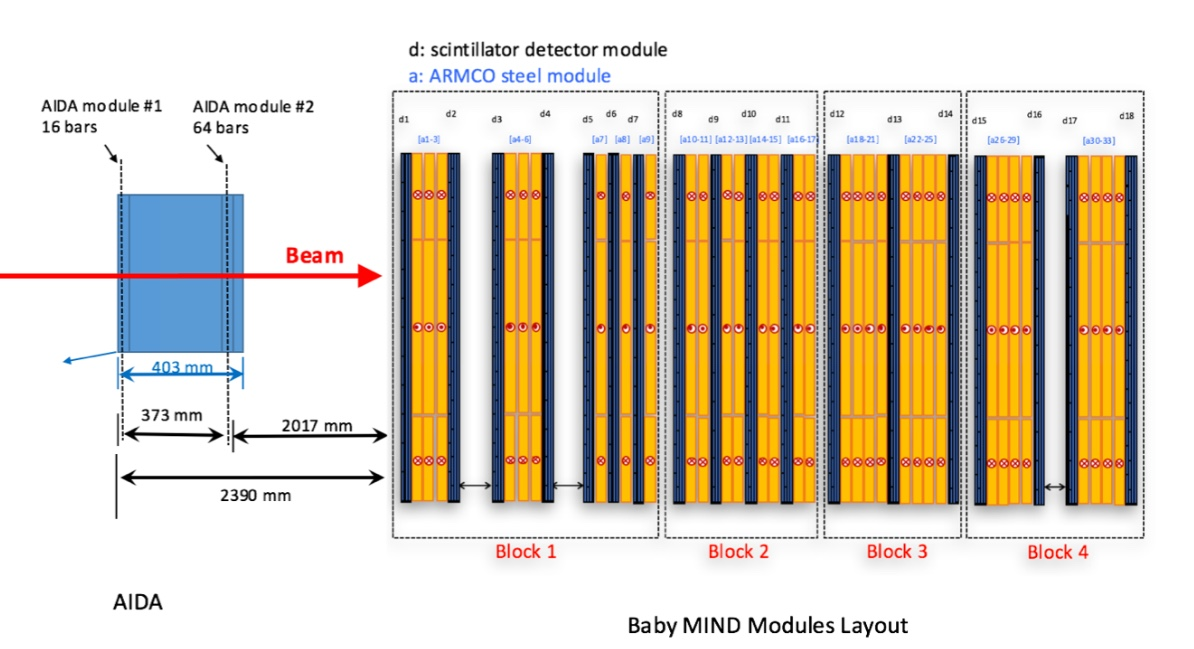
\includegraphics[width=\textwidth]{figures/MINDAIDAtestbeam.jpeg}
\caption{MIND in testbeam}
\label{fig:MINDtb}
\end{figure}

\subsection{Setup}

In order to support the magnets and scintillating modules mechanically, four support frames have been designed and constructed, specially to meet the transport requirements within CERN and while shipping to Japan. Baby Mind modules were installed in the four frames. Each block weighs about 20 tons which is within the operational range of the cranes at CERN and within limits for the transport containers to Japan.

A few meters upstream of the Baby MIND modules, AIDA modules were installed. These modules belonging to the project Totally Actice Scintillator Detector (TASD) are built from the same type of scintillating bars with 1 cm width, and same photosensors as Baby MIND. The AIDA modules were required to both provide a clear way of separating beam particles and cosmic particles as well as provide information about the incoming angle of the particle assumed and required by the reconstruction software.

 The particle signals in AIDA modules provide trigger signals for the arrival of beam particles, and also provide information about the incoming angle of the particles. A total of 44 FEBs mounted on 8 mini crates instrumented the 3996 channels of Baby MIND and 192 channels of AIDA.
All 44 FEBs were synchronized using the spill signal from T9 beam line which arrives one second before the arrival of the spill of particles. This signal was fed to a dedicated Master FEB on a separate MCR. The Master FEB would generate a reference clock signal for all the other FEBs acquiring data. The clock signal was distributed to 8 MCRs via three Fanout boards.

\subsection{Data preprocessing}
Similar to the previous test beam. Hits need to be converted into a test beam format.

Discuss how data was taken, what was done? Beam settings etc etc. What kind of simulations? Beam settings? Visualize the hits, see difference in expected curvature and spread. Many different reasons, electronics cosmics etc etc etc. Without hit amplitude this is very difficult.

Explain the full chain from how data is taken until it the analysis, results start.


\subsection{Analysis}

Compare momentum and spread. Mention that filters could be used to improve data. Momentum comparison, unknown real true momentum and particle ID. TMVA used to try to see if possible to separate and identify particle type. Describe also how it was trained, mention in section 4.

Show perhaps possibility in looking at single track events to identify showers vs muonlike particles. Also can see curvature and make an initial momentum guess based on it or based on the range if the event stops in the detector.


\subsection{Results}
Two of the main results provided during the test beam were both to commission the detector by showing that all parts works, including the reconstruction framework with hits in all of the modules and magnetic field providing the ability to estimate momentum. Results will be presented showing that the detector has been commissioned and showing that the reconstruction framework can read in this data and produce charge and momentum estimates for the beam.

\subsubsection{Data from unpacking}
Low level hits from only unpacking.

\subsubsection{Tracks from unpacking}
Using this data to build tracks.

\subsubsection{Hits in SaRoMaN}
Using unpacking hits, combined into 3d points in SaRoMaN. Use full simulation and digitisation framework


\subsubsection{Tracks in SaRoMaN}
Same way as simulate hits are used. Build possible tracks.


Mention efficiency and mention problem of not knowing beam composition. Handling pions.


\begin{figure}[h!]
\centering
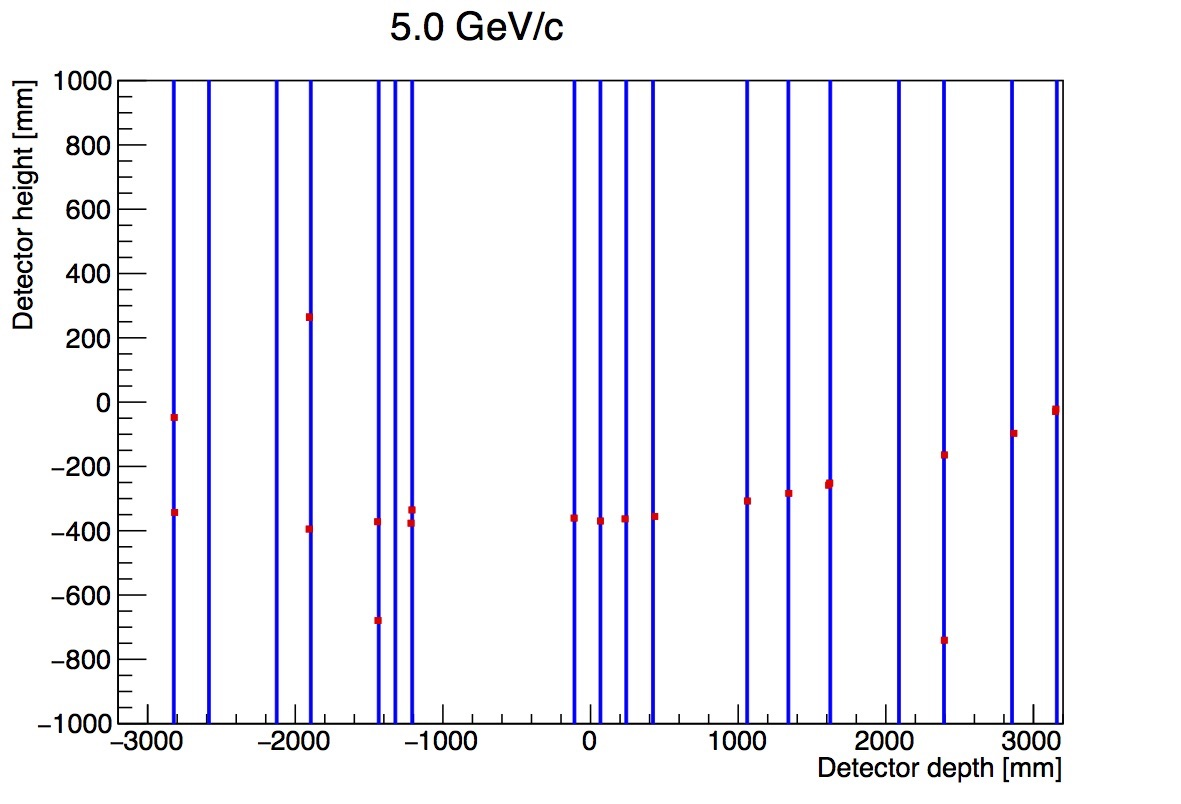
\includegraphics[width=0.49\textwidth]{figures/oldStudies/m5GeVevent2.jpg}
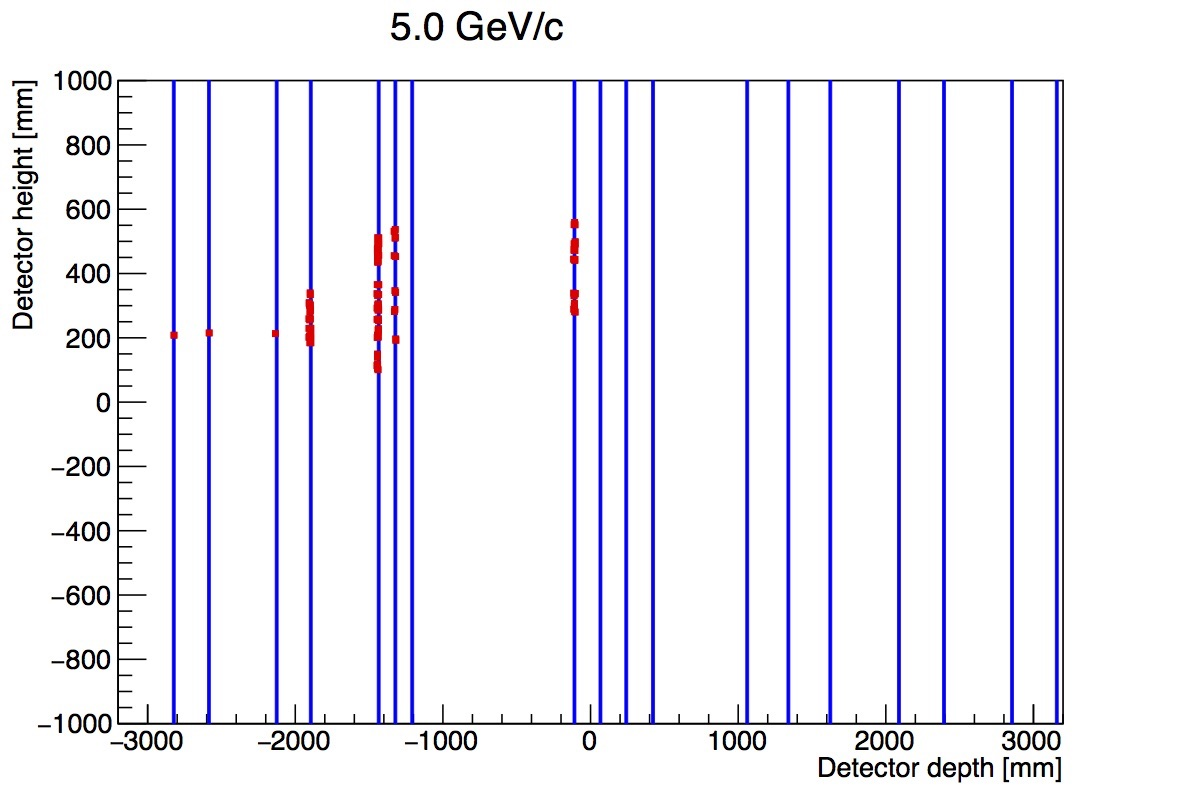
\includegraphics[width=0.49\textwidth]{figures/oldStudies/m5GeVevent3.jpg}
\caption{Sample events of test beam interactions at a set energy value of $5GeV/c$.}
\label{fig:EventsInitial}
\end{figure}

\subsubsection{Charge identification efficiency}

\begin{figure}[h!]
\centering
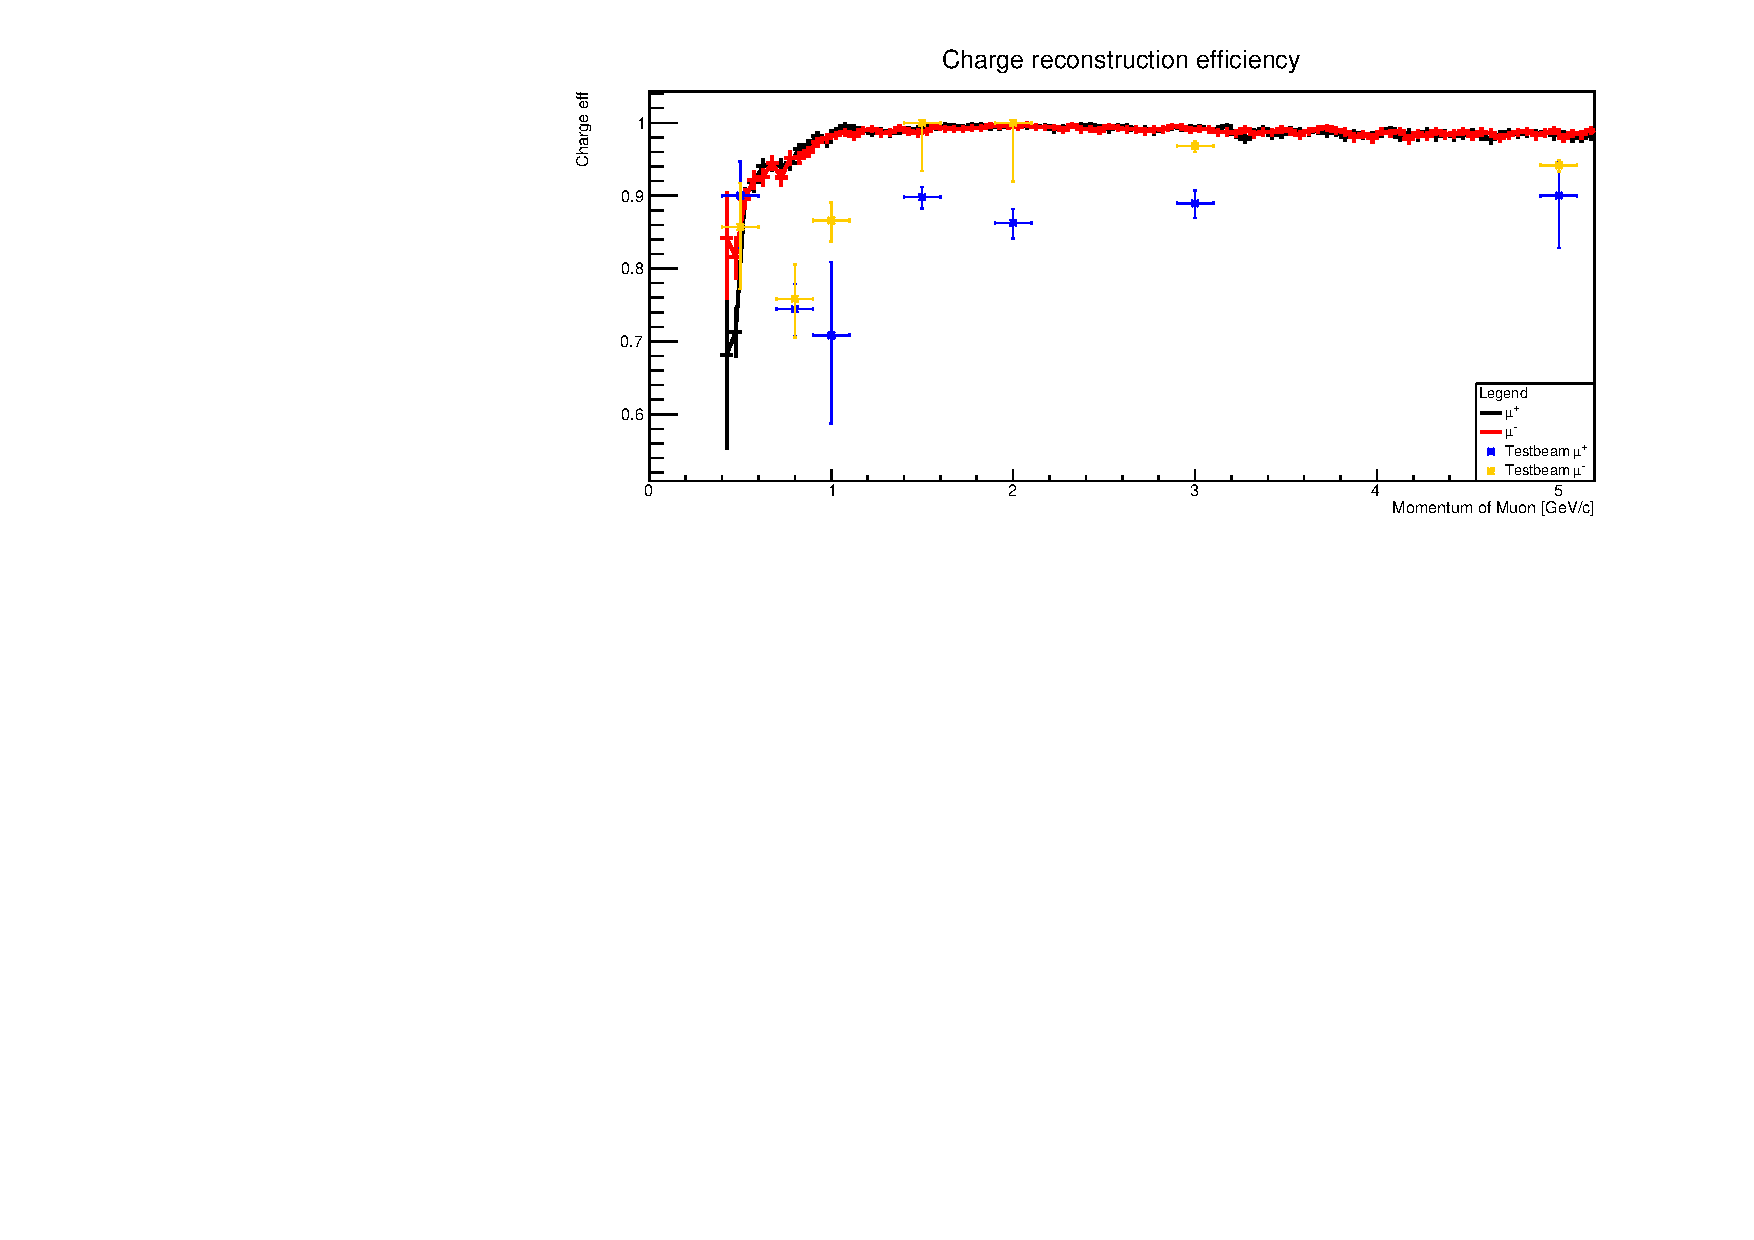
\includegraphics[width=0.49\textwidth]{figures/oldStudies/newChargeZoom5.pdf}
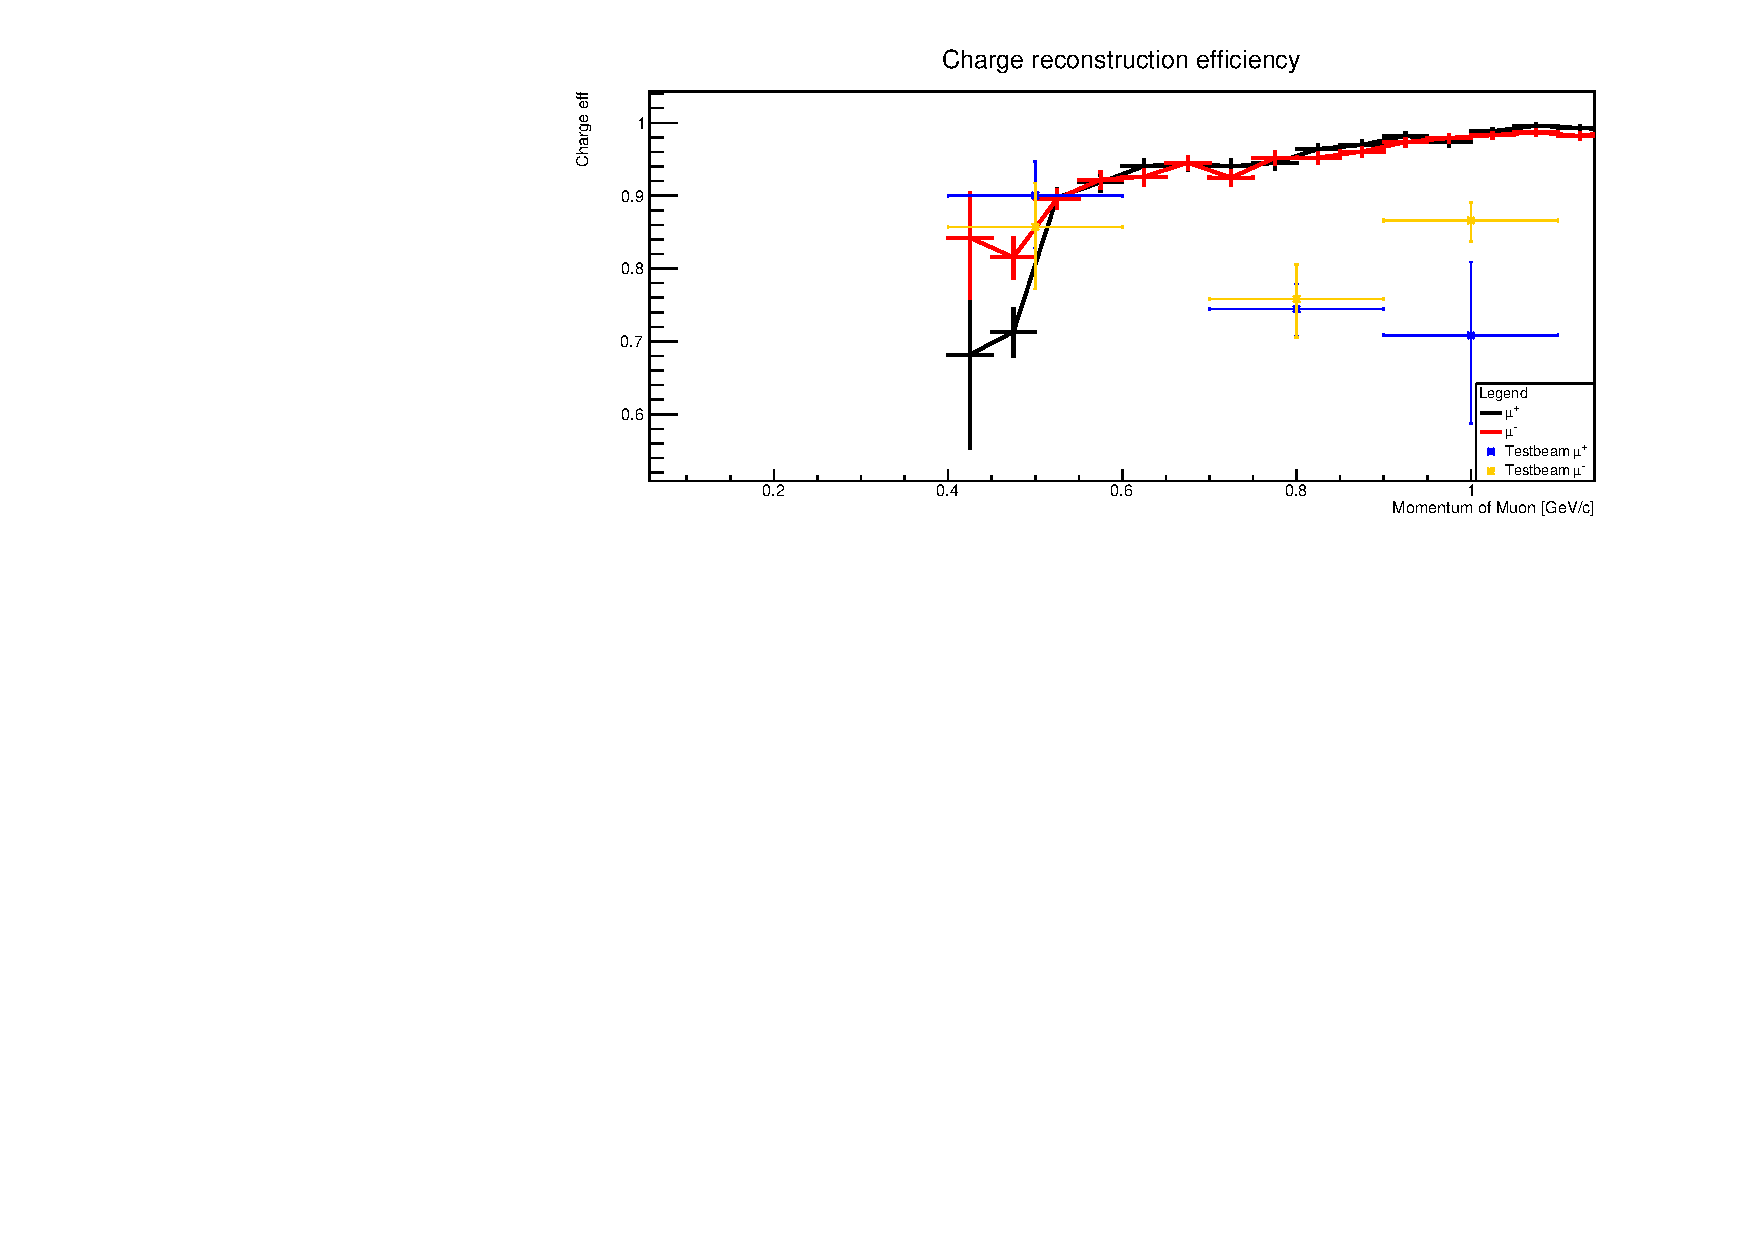
\includegraphics[width=0.49\textwidth]{figures/oldStudies/newChargeZoom1.pdf}
\caption{Initial charge id results}
\label{fig:ChargeInitial}
\end{figure}
Confirms that the full chain works and can produce plots, however the results are slightly less than expected. Add in event displays. Something to show both pion showers and muons. See expecting bending for first time! enough data to test recpack! Low pt and recpack ! Different regions.

Different run number? no real difference.

Improved unpacking gave more data.

\begin{figure}[h!]
\centering
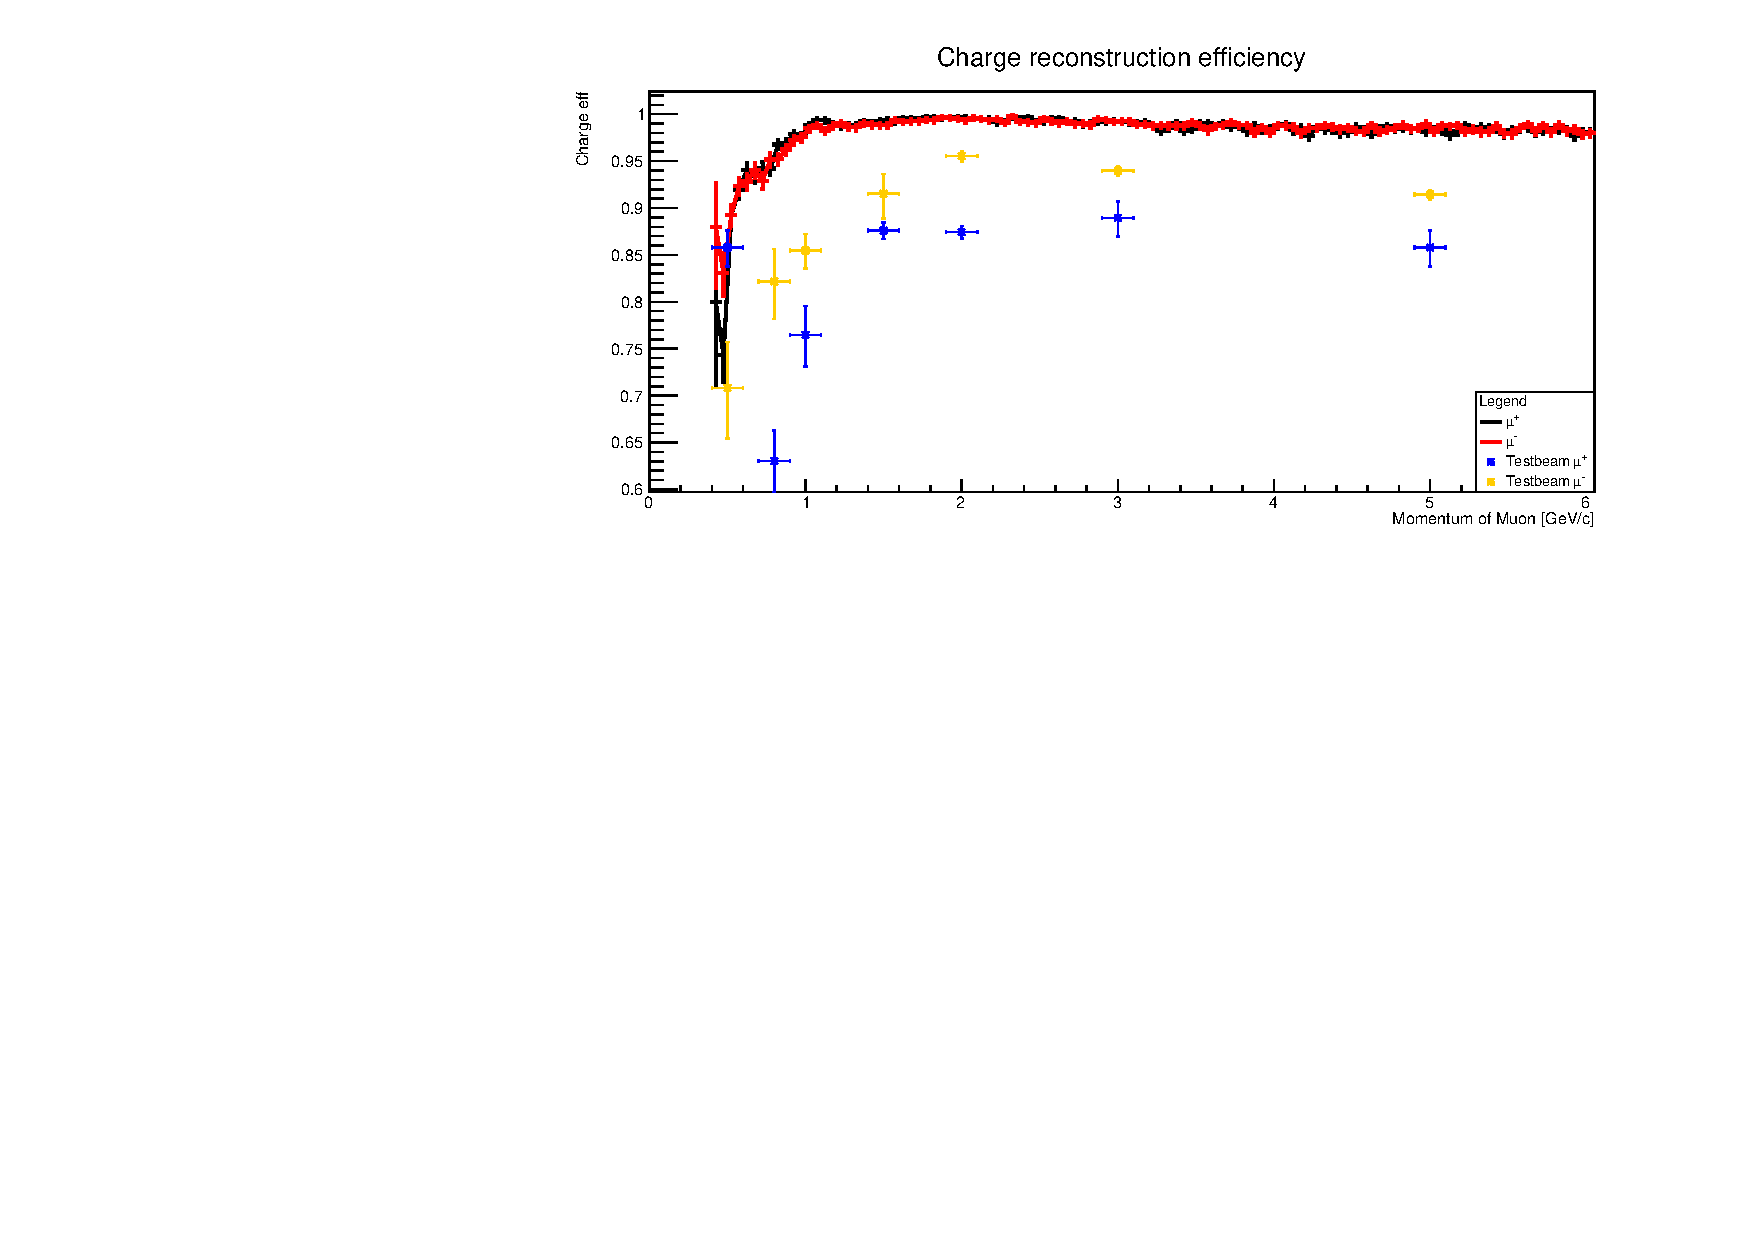
\includegraphics[width=0.49\textwidth]{figures/testbeam/TestBeam090318Plots/ChargeIDFull6GeV.pdf}
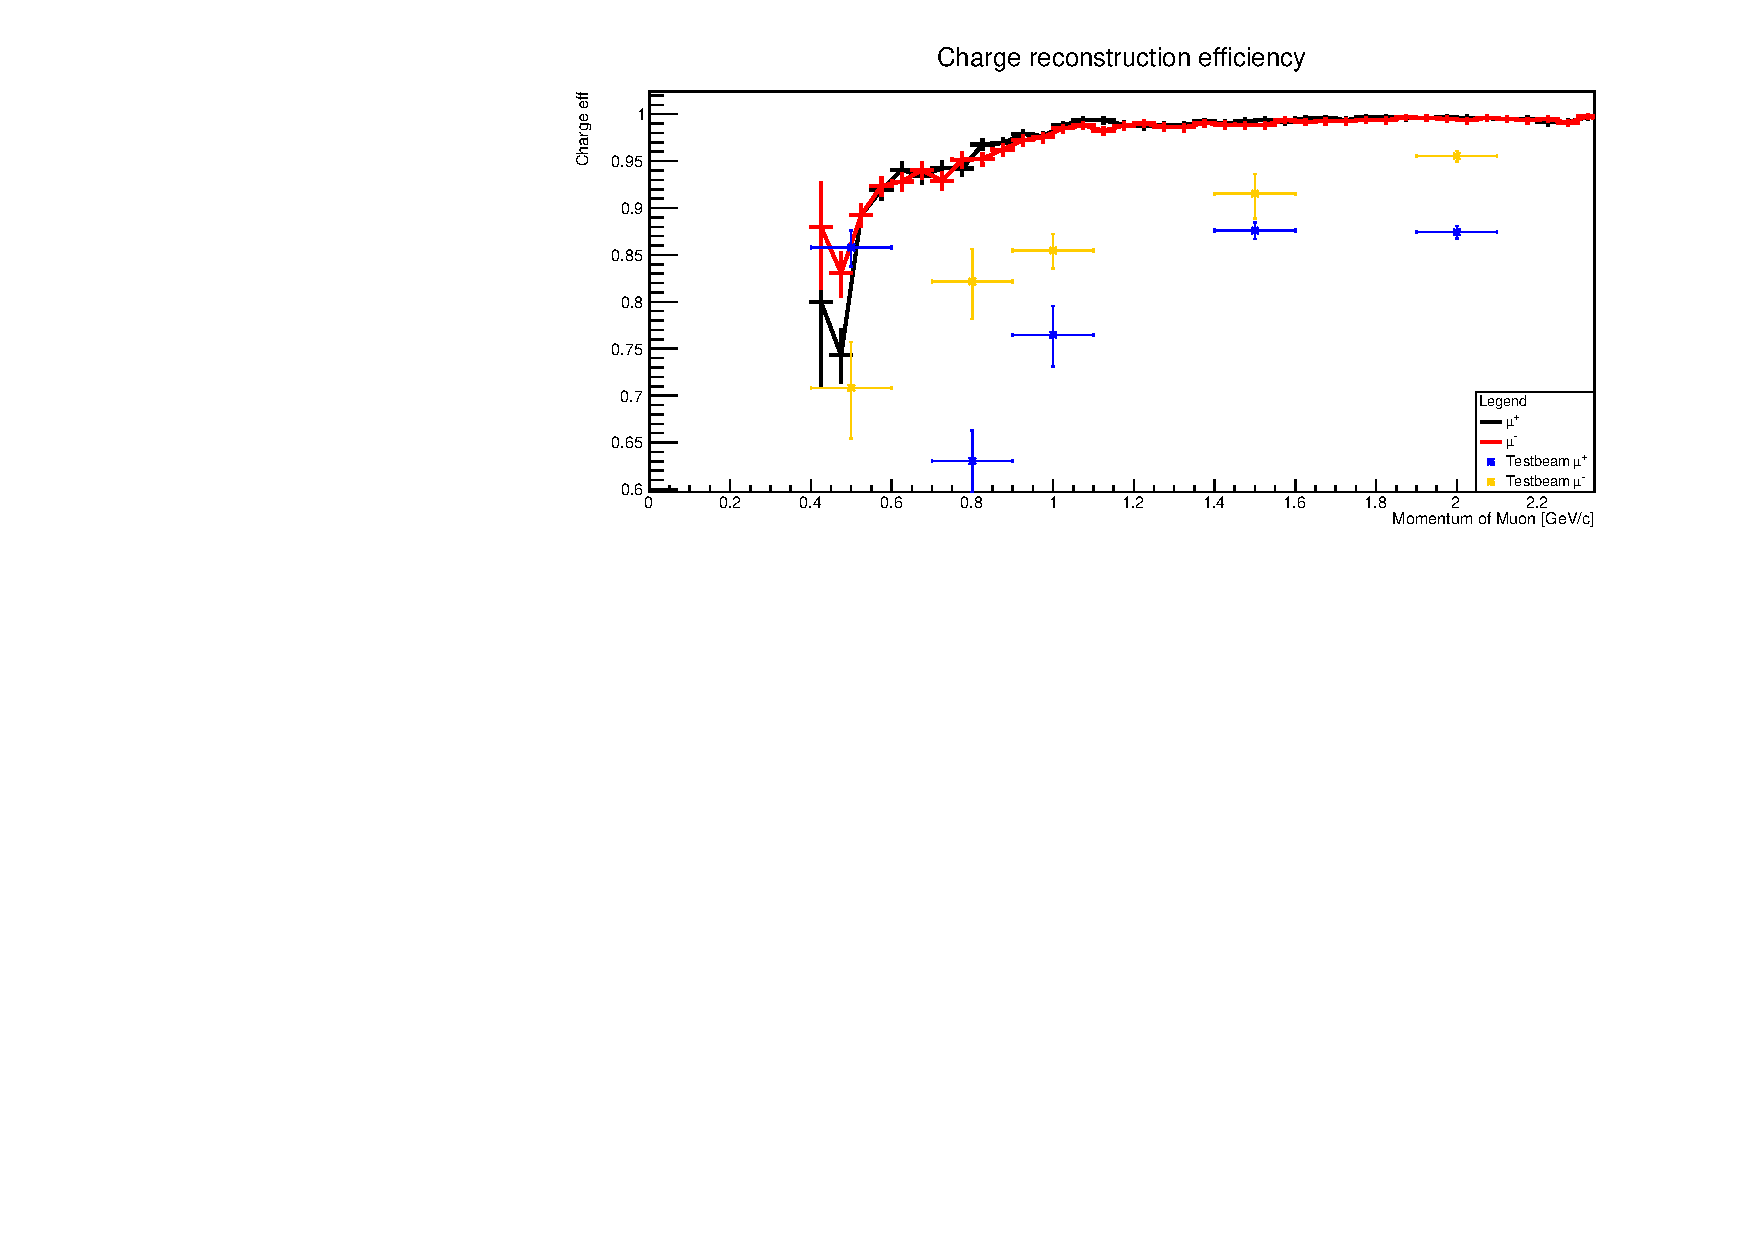
\includegraphics[width=0.49\textwidth]{figures/testbeam/TestBeam090318Plots/ChargeIDFullLow.pdf}
\caption{Initial charge id results}
\label{fig:ChargeImproved}
\end{figure}

Initial results, with pion contamination and initial unpacking. Discuss issue with cuts. Assuming that all hits had hit amplitude, unpacking could not collate hits correctly.

Confirm reconstruction even further. Will be able to properly run the code on the data.


Improving data (HOW?!?!) show similar result to previously. Slightly reduced errors etc etc. What about adding in expected reconstruction for pions? Show why we expect pion contamination or something else, but pion largest contribution known in t9 beam. 

Pion, almost all of them fall back onto final chance guess which fails badly. imagine it should be around 50\%. However, any pions in the sample would bring down the charge identification, even though we are trying to remove pions using cuts. Motivate PID with TMVA.

Motivating muon contamination in plots by comparing muon charge efficiency. Broken.

\begin{figure}[h!]
\centering
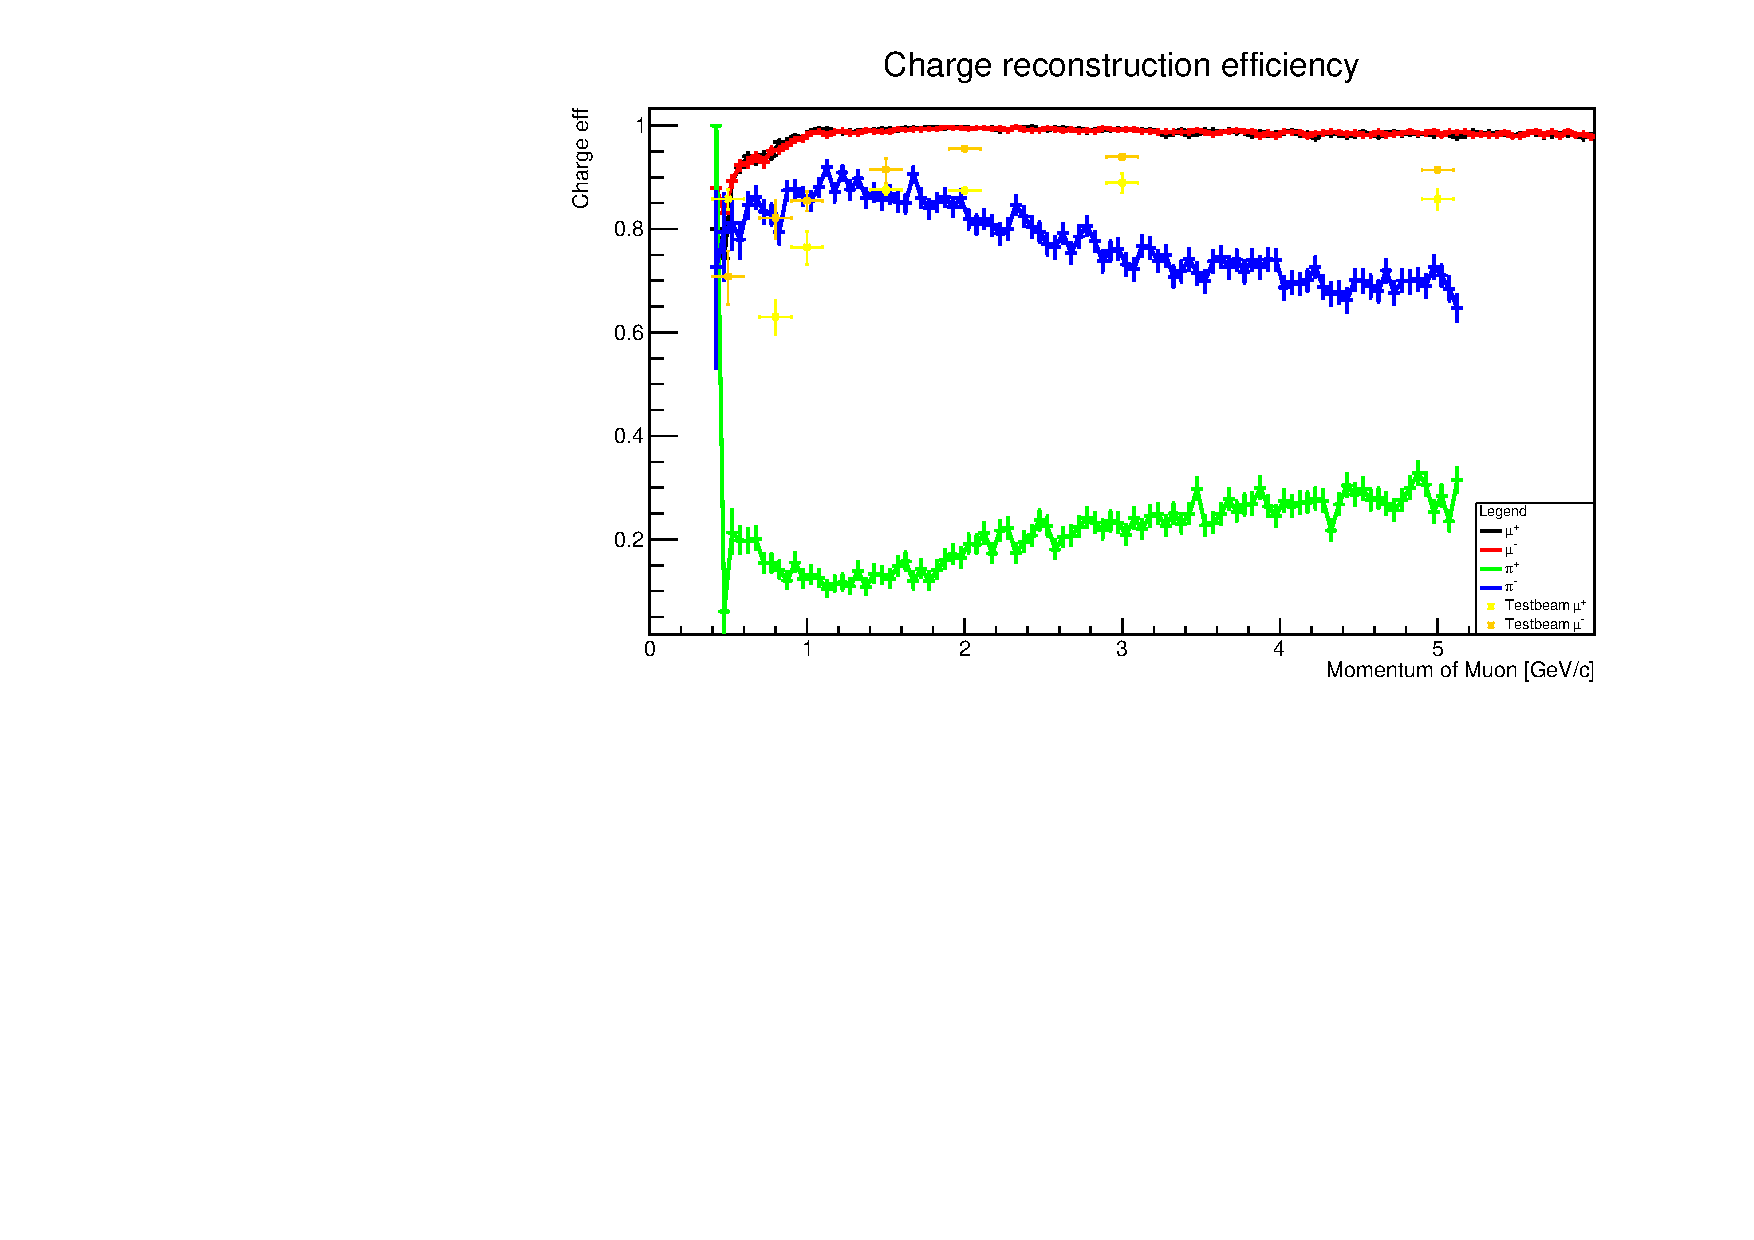
\includegraphics[width=0.49\textwidth]{figures/testbeam/TestBeam090318Plots/ChargeIDFullWPion.pdf}
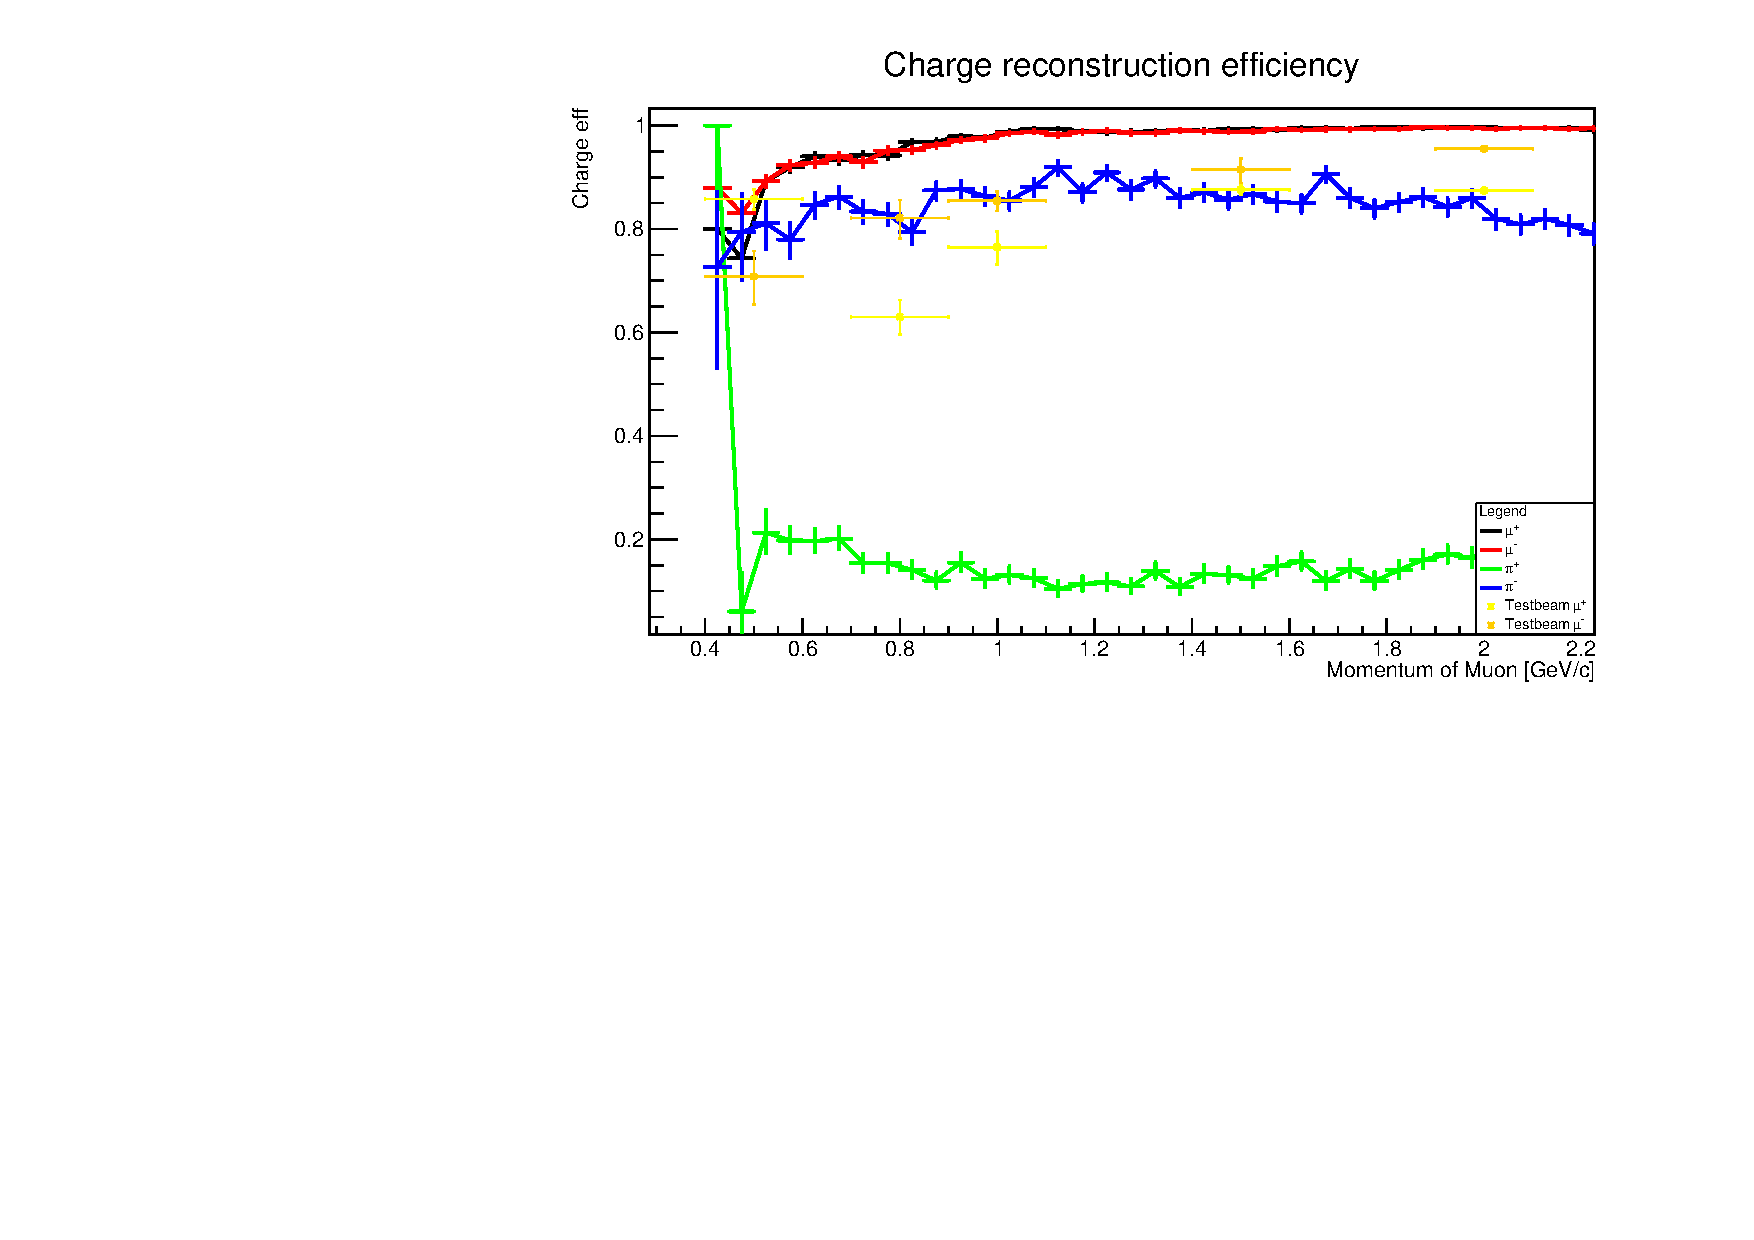
\includegraphics[width=0.49\textwidth]{figures/testbeam/TestBeam090318Plots/ChargeIDFullLowWPion.pdf}
\caption{Initial charge id results}
\label{fig:ChargeImprovedPion}
\end{figure}


Show most recent plots, which is the updated unpacking and more data, still issue comparing simulation to data. 

Use pion data to show how it may be possible that it is contamination. Charge ID for pion is low, reconstruction eff is also poor.

Reconstruction is defined as number of possible tracks in the software (more than 4 hits that produce a line) over tracks with a reconstructed momentum in the range $>0 and <\pm 10000$ i.e. a reasonable momentum. Charge takes these tracks and then checks charge.

Charge ID study momentum reconstruction. look at charge id for particles correctly momentum reconstructed, look after TMVA pID. 


Add details, not understanding what is correct data, further study has been performed but not solved problem efficiently. Unknown beam composition.


\subsubsection{Particle identification}

Using TMVA to classify muon from other events which may still pass through harsh criteria. 

Show plots of different simulated and TMVA in events with both muon and pion classification. Show loss of data, number in initial sample vs pion and muons after separation with efficiencies and values from training with all the appropriate plots.

Then provide final charge estimates and efficiencies.

This finally shows, that assuming the beam after this is sufficiencly pure there is a discrepancy between the simulations and final data representing detector and electronics factors which have not been taken into account. This also updates values provided from nufact and nuphys papers showing that the muon charge reconstruction is slightly lower than previosly thought. it is still better than 0 (T2K) and 0.6 or so from previous MIND type experiments. it is also possible to probe down to low energies which has not previously been possible.

\subsubsection{Momentum identification}
Discuss results and show the spread and difference between expected (put in by hand) simulations and measured distributions. 

Expected that the T9 beam area momentum is adjusted before final decay, actually choosing pion momentum and not muon momentum. Confirmed by email conversation. However, for lower momentum these match quite well. Large RMS from RecPack.



